\documentclass[11pt]{scrartcl}
\usepackage[parfill]{parskip}
\usepackage{graphicx}
\usepackage{booktabs}
\usepackage{tabulary}
\usepackage{float}
\usepackage{hyperref}

\graphicspath{{../images/}}

\title{\textbf{Project Management}}
\subtitle{Final assignment\\
            Release of a FLOSS product by a SME}
\author{Ricardo Garc\'ia Fern\'andez}
\date{\today}

\begin{document}

\maketitle

\vfill

\begin{flushright}
    \copyright  2013 Ricardo Garc\'ia Fern\'andez - ricardogarfe [at] gmail [dot] com.

    This work is licensed under a Creative Commons 3.0 Unported License.
    To view a copy of this license visit:
 
    \url{http://creativecommons.org/licenses/by/3.0/legalcode}.
\end{flushright}

\begin{figure}[h]
    \begin{flushright}	
        
\includegraphics{by}
        \label{fig:by}
    \end{flushright}
\end{figure}

\newpage

\tableofcontents

\newpage

\section{SME Introduction}
\label{sec:sme-introduction}

\par \emph{Code Garden} is our SME. We develop software products using quality patterns. Quality patterns are our main goal, applying Quality patterns to software development as is. plants and the code can not be kept alone, they can grow with life, diverted, or wither in a forgotten place. So plants like the code, need extra care, some gardeners, so they can grow and flourish. 

\par \emph{Technical Debt} is not a monster chasing us in every development sprint is another \emph{ROL} that we accept and we have interaction with it. We need him and he needs us.

\par Thus, we created a software product that helps us to deal with Technical Debt, \textbf{Greenhouse}.

\par \emph{Greenhouse} is our tool to track the progress of the evolution of code quality within a controlled environment. Using quality metrics for each programming language helps us reduce technical debt faster

\begin{quote}
    \begin{center}
    \emph{"we are the code we write"}
    \end{center}
\end{quote}

\par Increase productivity fighting against the technical debt of a project easily.

\begin{figure}[H]
\centering
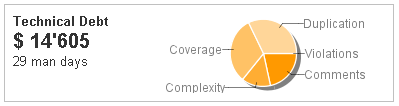
\includegraphics[width=0.7\textwidth]{sonar_technical_debt.png}
\caption{How much costs technical debt in your project ?}
\label{tech-debt-costs}
\end{figure}

% section sme-introduction (end)
\section{Publish the project}
\label{sec:publish-project}

\par We want to publish \emph{Greenhouse} as a FLOSS\footnote{Free Libre Open Source Software} project with two Software Licenses.

\par One a FLOSS License and the other a Private License. We chose a \emph{Dual-License} product.

\par Thus we can serve every type of costumers as MySQL business model explained by Elena Blanco\cite{dl-business-model}.

\begin{quotation}
    \emph{For anyone who wants to develop and distribute but does not want to release the source code for their application, MySQL is able to provide a commercial licence. Because MySQL has full ownership of the MySQL code, it is able to tailor its commercial licensing terms to meet the unique requirements of users interested in embedding or bundling MySQL.}
\end{quotation}

\subsection{Dual License}
\label{sub:dual-license}

\par Free Software License and Private, Brief discussion about licenses (your company has heard about some BSD or GPL, but they are not sure!).

\par FLOSS License selected to publish \emph{Greenhouse} is \emph{GPLv3}\footnote{GNU Public License Version 3 - \url{http://www.gnu.org/licenses/gpl-3.0.html}}. This FLOSS License provides \textbf{4 freedoms} to the project:

\begin{itemize}
	\item the freedom to use the software for any purpose,
	\item the freedom to change the software to suit your needs,
	\item the freedom to share the software with your friends and neighbors, and
	\item the freedom to share the changes you make.
\end{itemize}

\par The other License is a private License. A private License gives us more flexibility through market niche.

\par Good thing to take in advance using a Private License are:

\begin{itemize}
	\item Avoid possible or unexpected License Violations.
	\item Build a project in your company and be 100\% sure that you are not violation any License under your product.
	\item This License envelops the whole product into a private version.
\end{itemize}

\par This private License gives you the opportunity to deal with \emph{Greenhouse} libraries and include into other projects using full capabilities. This way you can avoid License problems with derivated works and be compatible with other FLOSS Licenses.

\par Brian Behlendorf\cite{brian-behlendorf-business-strategy} explains this model with a success and its weaknesses with the community development:

\begin{quotation}
    \emph{You have to be very careful, though, to make sure that any code volunteered to you by third parties is explicitly available for this non-free branch; you ensure this by either declaring that only you (or people employed by you) will write code for this project, or that (in addition) you'll get explicit clearance from each contributor to take whatever they contribute into a non-free version.}
\end{quotation}

\par We are very concerned about how to interact with the community. Our goal is provide to community the opportunity to develop solutions to our clients for \emph{Greenhouse}.

\begin{quotation}
    \emph{I would claim that if you treat your contributors right, perhaps even offer them money or other compensation for their contributions (it is, after all, helping your commercial bottom line), this model could work.}
\end{quotation}

\par Last quotation is how \emph{Transvirtual}\footnote{\url{http://www.transvirtualsystems.com/}} in Berkeley applied this model to a commercial lightweight Java. Encourage the developers to work and earn money directly with the software they make. We believe in this model to create a community involved around the product: 

\begin{itemize}
	\item The usability of the product.
	\item Tangible incentives as our case the money.
\end{itemize}

\par In this way we will try to solve the dilemma of FLOSS developments that can be converted into proprietary solutions.

\par Therefor, an exchange of knowledge by salaries to the community through an assignment of copyright to Code Garden by using the \emph{GPLv3 License}, they maintain the authoring and earn tangible rewards too.

\par We are the copyright holders of \emph{Greenhouse} and thus , we want to share the maintenability with community knowledge to provide solutions for companies with private Licenses of the product.

\par We want to evolve with the community and spread our developments and remain FLOSS.

% subsection dual-license (end)
% section publish-project (end)
\section{Market niche - Competitors analysis}
\label{sec:market-niche}

\par Code analysis is increasing everyday in software development. SME \& Big Enterprises focus its products near quality. Why ? Because Software Development is measurable, high measurable I could say. Every software is developed guided by patterns through developers and the final product (talking about clients) is released to the client showing its functionality but what happens with all the code developed inside ?

\par The code evolves as the development grows. In a development team is difficult to measure the quality of the product grained.

\par Other sample of the use of measure the quality is when you have to choose between two libraries to implement another service that use the functionality implemented by them. One metric to take care is the code quality that you can apply for them. Using some objective metrics you can retrieve a numeric result that gives you a general idea. Or if you want to add an existing module/library you can choose the one which its result is near to your software, not lesser not higher. It is a way of seeking for a balance in development and knowledge about complexity of a module to import to your product.

\par There are some samples of Analyzing tools but we are to analyze \emph{Code Climate} and \emph{Sonar}.

\subsection{Code climate}
\label{sub:code-climate}

\textbf{Code climate} - \url{https://codeclimate.com/}. Code quality analysis in Ruby Language. But we will not focus on language but with what gives us the tool in Figure~\ref{code-climate}.

\begin{figure}[H]
\centering
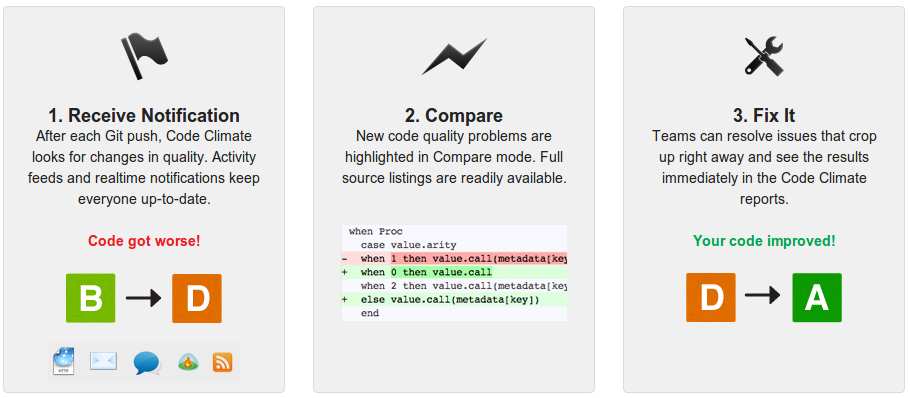
\includegraphics[width=0.7\textwidth]{code-climate.png}
\caption{Code Climate Notifications}
\label{code-climate}
\end{figure}

\par This tool gives us interoperability with Software Forges like Github integration. Source Code Management with Git repositories, Code Quality evolution, Notifications, Comparison tools. This tool set is simple but efficient, this is very important. Play with the ease of integration into a forge development offering hosting server, pay and enjoy the product (one click purchase).

\par Includes the main features of services; \emph{PaaS}\footnote{Platform as a Service}, \emph{IaaS}\footnote{Infrastructure as a Service} and \emph{SaaS}\footnote{Software as a Service}. Using \emph{bluebox services} - \url{https://bluebox.net/}: Virtualized Environments on Actual Hardware.

\par We want those services available for every developer and easily result visualization.

\par It's \emph{free (gratis)} for FLOSS projects.

% subsection code-climate (end)

\subsection{Sonar}
\label{sub:sonar}

\textbf{Sonar} - \url{http://www.sonarsource.org/}. Sonar slogan is very clear:

\begin{quote}
    \emph{Put your technical debt under control}
\end{quote}

\par Despite Code Climate, Sonar covers lots of languages and is a FLOSS product. A very good point to consider for the use of this software. Controls and test every corner of your project in Figure~\ref{sonar7axes}.

\begin{figure}[H]
\centering
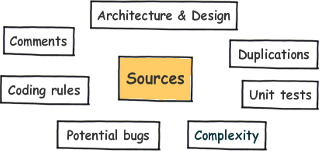
\includegraphics[width=0.7\textwidth]{sonar7axes.png}
\caption{Sonar covers 7 axes}
\label{sonar7axes}
\end{figure}

\par This Software gives you the opportunity to integrate with your Source code management and a result metrics result visualization panel with Nemo (in Figure~\ref{nemo-evolution}) - \url{http://nemo.sonarsource.org/} using Saas solution through \emph{Cloud Bees} - \url{http://www.cloudbees.com/platform-service-sonarsource.cb}.

\begin{figure}[H]
\centering
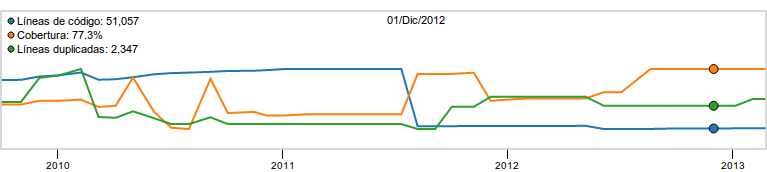
\includegraphics[width=0.7\textwidth]{nemo-evolution.png}
\caption{Nemo evolution graph}
\label{nemo-evolution}
\end{figure}

\par Sonar is focused in code Analysis its market niche as Code Climate but offering easy configurable solutions for integrate your projects with giving you the possibility to analyze our software and visualize the results among time.

\par This is our niche, Software Analysis, visualization and interoperability between Source Code Management.

% subsection sonar (end)
% section market-niche (end)

\section{Management general path}
\label{sec:management-path}

\par Communities, Enterprise ROLE, Single Vendor or Apache Software Foundation.

\par We want an open community starting from basic decisions and fast information spread, not noise, information. We need to know \emph{what kind of community we want to be}.

\par From this reason we have to establish the basic guidance and scalability rules. Our first step is to publish the code with Dual-License (FLOSS and private). Yes, the license matters in every community.

\par Our starting community is composed by our development team from \emph{Code Garden}. Two developers that have been developing the project. We invest the knowledge and their work hours into this community project because we bet to improve from a community. We are not searching for a direct revenue. They take the role 'without' company brand because we want a community. 

\par The brand of the company has to become the solution for the project \emph{GreenHouse} and related projects doing networking with other communities. Because of that we need three ROLES:

\begin{itemize}
	\item Community Manager.
	\item Technical Developer.
	\item Company behind the project inspiring confidence.
\end{itemize}

\subsection{Community Manager}
\label{sub:community-manager}

\par One of them has to take the ROLE of the Community Manager. This ROLE is in charge of the communication, promoting, technology, development, interviews and pro-active person inside our company and the community. We need a bridge between our community, clients and our company to learn from distinct points of view. Our goal is that the Community Manager will be associated to \emph{Code garden}. So to raise this we have to give him visibility through internet channels: company website, company blogs, personal blog, social network (SME and project) and try to guide the community developers to he.

% subsection community-manager (end)

\subsection{Technical Developer}
\label{sub:tech-developer}

\par The ROLE of the \emph{Technical Developer} is that he has to be known inside the developers community, the part of the community that contributes with code. Has to be a clear person, pragmatic and open-minded. Take the ROLE of a \emph{Benevolent Dictator For Life}\footnote{\url{http://www.artima.com/weblogs/viewpost.jsp?thread=235725}} as \emph{Guido Van Rossum} was baptized by one of the attendees at a lecture in 1995.

\begin{quotation}
    \emph{"I believe I've tracked down the origin of the term Benevolent Dictator For Life (BDFL) to a Python meeting in 1995. It's a blast from the past!"}
\end{quotation}

\par This person is charge of project development as a project manager in an \emph{Enterprise Language} but more open minded to their community members. Is the \emph{'creator'} of the project and deserves a higher degree of credibility on issues directly related to the project.

\par We need one, but we don't want one for the eternity because our goal here is that the community manages the project and grows horizontally. \emph{Kill your idols, be yourself} that's the goal here.

\begin{figure}[H]
\centering
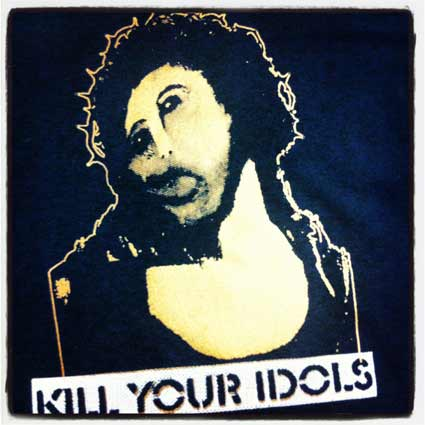
\includegraphics[width=0.7\textwidth]{killyouridols.jpg}
\caption{Ecce Homo - Kill Your Idols}
\label{kill-your-idols}
\end{figure}

% subsection tech-developer (end)

\subsection{Enterprise ROLE}
\label{sub:enterprise-role}

\par Enterprise ROLE is the most important at the beginning because \emph{Code Garden} is the copyright holder of the project. \emph{Code Garden} is the \emph{'authority'} in this project and has to change its ROLE acting between a Community Manager and Solutions Provider Expertise for this project and related projects for manage Technical Debt.

\par Our goal is to become an \emph{Expertise Enterprise Managing Technical Debt} not only \emph{GreenHouse}. The project transition from private to public and job opportunities to community members contributing with solutions to our clients.

\par We have to transform the lonely project into a \emph{Community Driven Project} and incentive our clients to enter to the community, reading, sharing, contributing (everything not just code). We need the company to create a solid and professional support to the project. Use the project and show the results, convert strange numbers into easy coloured graphs. Work as a company that is guiding its business model into FLOSS.

% subsection enterprise-role (end)

\subsection{Social and political organization}
\label{sub:social-political}

\par The social and political organization of the project must be horizontal. Decisions have to be complete through the transparency and the participation of members of the community.

\par We are going to use Apache Software Foundation ways of decision making\footnote{\url{http://community.apache.org/committers/decisionMaking.html}} verbatim:

\begin{itemize}
	\item \emph{Lazy Consensus} - Lazy consensus is the first, and possibly the most important, consensus building tool we have. Essentially lazy consensus means that you don't need to get explicit approval to proceed, but you need to be prepared to listen if someone objects.

	\item \emph{Consensus Building} - Sometimes lazy consensus is not appropriate. In such cases it is necessary to make a proposal to the Mailing List and discuss options. There are mechanisms for quickly showing your support or otherwise for a proposal and building consensus amongst the community. Once there is a consensus people can proceed with the work under the lazy consensus model.

	\item \emph{Voting} - Occasionally a \emph{"feel"} for consensus is not enough. Sometimes we need to have a measurable consensus. For example, when voting in new committers or to approve a release.
\end{itemize}

\par \emph{Lazy Consensus} is \emph{the most consensus building tool we have} (as ASF said) to guide a community from the beginning. Because you don't need community approval but you need to be prepared to listen if someone objects. Community has to reach consensus if a contrary view argued over the solution to develop. This opens us to another door, do-cracy 

\par Consensus building appears when lazy consensus steps in a contrary argued opinion, so we have to reach a consensus between two (or n) parts. Another use is to prepare a new feature, fix a bug, new release, discontinue a development, create a new communication channel, do a workshop. The community has to be horizontally guided and consensus build. For these direct consensus in communities we need to merge consensus and voting tools into one to reach the maximum number of people through votes.

\par Voting tool is very important tool used mixed with two consensus types. We need to know something from the community, we want an opinion, an answer, etc\ldots The most important things are preparing the votes and explain the rules, so explain the voting rules clearly. Using ASF\footnote{\url{http://community.apache.org/committers/voting.html}} guide we have 3 vote types:

\begin{itemize}
	\item +1 Yes I agree
	\item 0 I have no strong opinion
	\item -1 I object on the following grounds
\end{itemize}

\begin{quote}
    \emph{If you object you must support your objection and provide an alternative course of action that you are willing and able to implement (where appropriate).}
\end{quote}

\par Objection and its process is very important because if you are not agree with a proposal you must to implement and argue your why.

\par These social-political guidelines aim the community to be more participative, respectable and reasonable through a rational perspective. When provide rational solutions (argued in favour of the common good) is when more is learned and enjoyed discuss.

% subsection social-political (end)

% section management-path (end)
\section{Management Policies}
\label{sec:management-policies}

\par Linking with the previous section \emph{Social and political} organization now we are focused in management, how to and which channels are necessary to develop these organization management applying strategies.

\subsection{Where will be published the code ?}
\label{sub:publish-code}

\par First is not where, first is, which SVC - \emph{System Version Control} - will be used ?

\par We choose a DVC - \emph{Distributed Version Control} - System instead of an CVC\emph{Centralized Version Control} System. A \emph{DVC} increases the capabilities to developers (including community contributors) to develop solutions and test their development in every environment. The main reason is that a \emph{DVC} gives you the opportunity to work without being connected to internet and save all your historical revisions. The other reason is that applying \emph{DVC} Systems (mainstream) workflow Branch per Feature from Martin Fowler analysis\cite{branch-per-feature} and how to fit with Continuous Integration Development, increases the productivity and facilitates the integration of new developments minimizing the problems with merging in \emph{CVC}s. Thinking about publishing a project as FLOSS with the idea of creating a solid and integrate community we must use a \emph{DVC}.

\par The are different \emph{DVC}s to choose:
\begin{itemize}
    \item Monotone - \url{http://www.monotone.ca/}. monotone is a free distributed version control system. It provides a simple, single-file transactional version store, with fully disconnected operation and an efficient peer-to-peer synchronization protocol. \emph{Introduced hash commits}.
	\item GNU Arch - \url{http://www.gnu.org/software/gnu-arch/}. It is used to keep track of the changes made to a source tree and to help programmers combine and otherwise manipulate changes made by multiple people or at different times.
	\item Bazaar - \url{http://bazaar.canonical.com/en/}. Bazaar is a version control system that helps you track project history over time and to collaborate easily with others. \emph{GNU Arch fork}.
	\item Darcs - \url{http://darcs.net/}. Darcs is a free and open source, cross-platform version control system, like git, mercurial or subversion but with a very different approach. Thanks to its focus on changes rather than snapshots, Darcs can offer a freer way of working, and a simpler user interface. It's written in \emph{haskell}.
	\item Git - \url{http://git-scm.com/}. Git is a free and open source distributed version control system designed to handle everything from small to very large projects with speed and efficiency.
	\item Mercurial - \url{http://mercurial.selenic.com/}. Mercurial is a free, distributed source control management tool. It efficiently handles projects of any size and offers an easy and intuitive. 
\end{itemize}

\par After a deep analysis for choose one \emph{DVCs}. We decided to use Git. Our decision is based in the facility to propagate through internet, most development forges allow and promote the use of Git instead of others, this could be a hype but a hype that works because if this system has not a good \emph{interoperability} APIs and easy hooks configurations will be replaced easily. And was born from Linus Torvalds after BitKeeper affair with taxes and its 'special' license clause\footnote{\url{http://kerneltrap.org/node/444}} to manage Linux kernel source.

\par After choosing Git we must decide where. We decided to host our Git Repository in Github - \url{https://github.com/} - Projects and community in Github have a lot of visibility and uses a clean user-friendly interface furthermore is a Git powered forge that allows an easy implementation of hooks to our repositories. Why is this important to us ? Because our project is a code analyzer, where could be better hosted to be tested than in an easily interoperability configurable forge that spread hook integration? I think this forge increases the visualization to our work, organization capabilities and community communication, the most important issue. 

\par GitHub has an easy patch/merging/pull-request tool to merge work from contributors, using code visualization, comments in commits and patch visualization. It's very easy to apply a contribution. Furthermore gives to the project set of quick analysis graphs from contributors commit activities and branch history, these analysis are a key feature to gain visibility for the community in Figure~\ref{github-graphs}.

\begin{figure}[H]
\centering
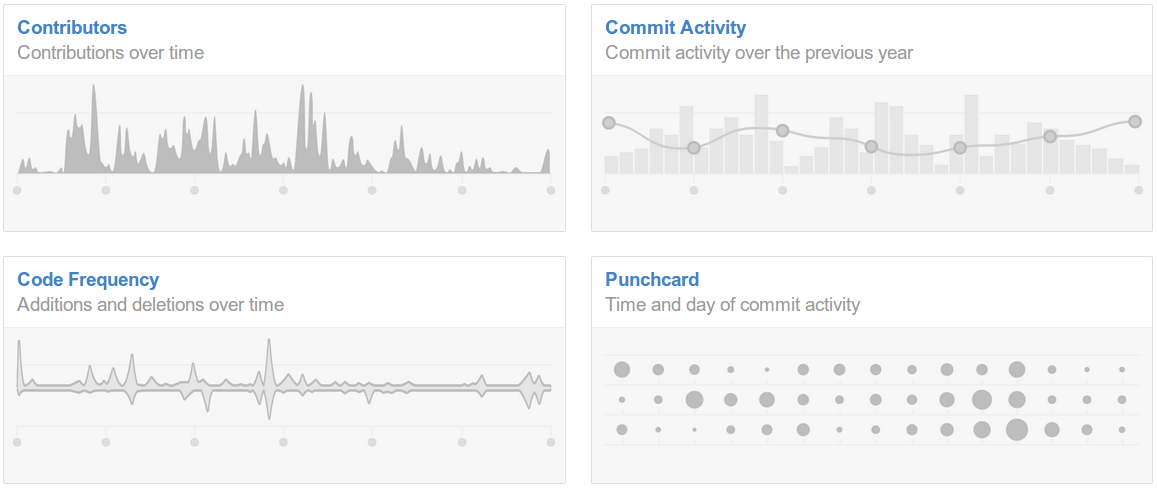
\includegraphics[width=1\textwidth]{github-graphs.png}
\caption{GitHub contributors graphs}
\label{github-graphs}
\end{figure}

% subsection publish-code (end)

\subsection{Communication strategy and channels}
\label{sub:communication-strategy}

\par In communication staging we have to accomplish with two main groups: \emph{strategy} and \emph{channels}.

\par Starting with \emph{Jono Bacon}\cite{art-of-community} introduction to \emph{Communicating Clearly} chapter:
\begin{quotation}
    \emph{"Community is absolutely about understanding the ether. Our notes are the processes, governance, tools, and methods in which we work together. The notes we don’t play are the subtle nuances in how we pull these notes together and share them with one another. The space between the notes is communication."}
\end{quotation}

\par Stands as the centrepiece of his chapter, the most important thing in communication within a community are \emph{"the notes you do not play"}, citing a quote from Eric Clapton. That is, when we know which is the vehicle we need to introduce for proper communication. It is more important that we miss something than overcharge the channels

\par Therefore, we will divide the process into two phases. Using the analogy of the roads and driving through them we have:
\begin{itemize}
	\item Create the highways - Channels: such as Mailing lists, forums, and discussion channels.
    \item Encourage great driving - Strategy: providing a consistent example of simple approaches to communication that make the community easier to understand and more pleasurable for everyone involved)
\end{itemize}

\par Thinking about our project, \emph{Greenhouse} is a technical project for technical users. This is the first step to choose an appropriate channel. We have developers in our company and first users (that could became developers) thus we want to separate the communication between two channels:

\begin{itemize}
	\item Mailing lists: Create different Mailing lists for each type of subscriber: developer, user. 
	\item Forums: Forum to get an easy human enter door to the project for a newbie developer and not expecting to be the main communication channel.
\end{itemize}

\subsubsection{Mailing Lists}
\label{sub:mailing-lists}

\par Be clear, specific and human (the most important). In Mailing Lists we have to be in touch with the people interested to contribute to the project, not only the short term upstream, we are focused in long term upstream. Thus we have to be organized, focused and good mates. \emph{Mailing Lists} will be public and this has to be in the whole project, because of transparency we can create a trustful community around the project.

\par Starting with mailing list, we need a clear language, follow Netiquette\footnote{\url{http://tools.ietf.org/html/rfc1855}} basic guidelines and respect everyone’s opinion. 

\par Avoiding the main problems in Mailing List such \emph{bikeshed}\footnote{The gist is that while nobody will question the details of a large and complex project (e.g. a nuclear reactor), for a simple thing as a bikeshed everybody will loudly add their two cents as to exactly how it should be built/painted/constructed} and over technique discussions which can drive away new community members.

\par \emph{Mailing Lists} have to be maintained and guided by the community thus we have to be clear and describe process, guides and documentation.

% subsubsection mailing-lists (end)
\subsubsection{Forums}
\label{sub:forums}

\par The \emph{Forums} create a friendly user interface for a newbie users to get in touch with community and little problems that couldn't fit well in our \emph{Mailing Lists}. Gives the opportunity to search and reply easily. To the new user or the user that only is looking for one determinate question, such as FAQS\footnote{Frequent Ask Questions} or version release posts.

\par \emph{Forums} maintenance could be assumed by a developer (in the beginning) and other forum users that increase its participation and rank by meritocracy inside the \emph{Forum}. The purpose of the forum is to be handled by community to introduce a friendly-human face to newbie users.

% subsubsection forums (end)

\par After chose these \emph{"highways"} and \emph{"Encourage great driving"} we need documentation, clear documentation related to this tools. How to get started and how to choose the right \emph{"highway"}. This will guide the user (pre-community user) into the channels and facilities of community. 

\begin{itemize}
	\item Where are the tools ?
	\item How to start. Firs search, is not necessary to be register to search for information. Transparency and increasing engagement with the community interacting.
	\item Guides and rules to write, showing samples. Friendly and human samples. For the administrator and the basic user.
	\item FAQs - Resolved issues, HowTo's, help and where is.
\end{itemize}

\par Furthermore we have to use blogs, create and produce content related to the community, personal blogs, technical blogs, articles, stories about the community, talks and success cases. This could be another highway to spread information about the community and the project.

\par If you are looking for IRC channel, you won't find it. We started this section referring us to the appointment of Jono Bacon \emph{"the notes you do not play"} therefore we decided not to create an IRC Channel for the community because we can't manage it whit our resources. Ff the community will want one we will be happy and could try to afford this cost in the future.

\par I want to include a reference to Issue Tracker System (ITS) in this section as a \emph{highway} and \emph{encouraged driving} element. The \emph{ITS} is important in a community, in our case a technical community not focused in an end-user. We include an \emph{ITS} to manage the project in the community, communications, RFC - \emph{Request For Comments}, Doodles, discussions, documentation, references and of course \emph{Netiquette} related to how to use an \emph{ITS} which is explained widely in Technology Section\ref{sec:technology}.

\par This tool is the jump for the user after the \emph{Forums} and \emph{Mailing Lists} to contribute to the development aimed by the members of the community. Following Netiquette guidelines to post a bug into the \emph{ITS} and stay tuned with issue updates, test the patches and help developers to fix any bug.

\par Because of is another communication channel with development team I chose to reference the \emph{ITS} inside this section.

% subsection communication-strategy (end)

\subsection{Managing volunteers and attracting new users}
\label{sub:volunteers-users}

\par \emph{Managing volunteers and attracting new users} is \textbf{the million dollar question}. How do I attract new users ? and more difficult; How should I do to manage volunteers? How should I do to avoid losing them?

\par Our project is based on the excellence of the code, the fight against technical debt that always creeps into projects. On this basis, every developer wants to develop good projects. Based on studies of refactoring and code quality from the book Refactoring by Martin Fowler\cite{refactoring}, somehow we want to teach and develop better code using this tool. Furthermore the easy result visualization of the results and evolution of the code. The tools to \emph{increase and spread} visualization of the results and \emph{how to} are explained in Technology section\ref{sec:technology} to attract new users.

\par This attract every developer and company that want to work better easily. This is the technical hook.

\par But we have to focus to the community hook and how to keep volunteers inside the project.

\subsubsection{Managing volunteers}
\label{sub:volunteers-management}

\par \emph{We want users} because the users could \textbf{become contributors}, so this door is the first step to create a community. Following the \emph{Onion Model} in Figure~\ref{onion-model} defined by \emph{Kevin Crowston} and \emph{James Howison}\cite{social-structure-floss} after studying \emph{120 FLOSS projects} looking for a community pattern in communication centralization, they found the onion model structure.

\begin{figure}[H]
    \centering
    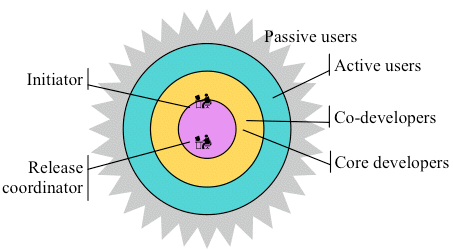
\includegraphics[width=0.7\textwidth]{onionstructure.png}
    \caption{Onion model}
    \label{onion-model}
\end{figure}

\par From \emph{passive users} that are in the corner of project through \emph{active users} that could become \emph{co-developers} or not. And finally \emph{core developers}. Furthermore we must comprise the role jumps that can occur between the different strata of the community that was explained by \emph{Jennifer Preece, Ben Shneiderman} communities study\cite{preece2009reader} represented in Figure~\ref{reader-to-leader}.

\begin{figure}[H]
    \centering
    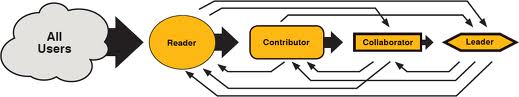
\includegraphics[width=1\textwidth]{reader-to-leader.jpg}
    \caption{Reader to Leader}
    \label{reader-to-leader}
\end{figure}

\par These Volunteers workflow inside communities depends on the community, so we want to give opportunities to new users with easy feedback from the community and vice versa. Know how are they, why they want to contribute, but not directly, nobody answers to a question directly without knowing nothing about the other people. We need to create a trustful circle, not about trust epic trust, a circle open to collaboration giving confidence to self-organization inside the community. Participate by him/herself.

\par Promoting the users into different levels in the project to share a complete view of the community. The ROLES could and should change. \emph{Pro active community core creates pro active community members}.

\par Remembering volunteer management, we again seek help at work, offering work to the community users to collaborate on the project and receive financial remuneration. Working as a community to benefit from it. In the first instance you will get the benefit per individual, we will explain how to scale these revenues this in the future into the community.

\par And of course, this community badges by meritocracy\footnote{Oxford Dictionary: Government or the holding of power by people selected according to merit} have to be obtained from data. This has been explained in technology section\ref{sec:technology} tool by tool.

% subsubsection volunteers-management (end)

\subsubsection{Attracting new users}
\label{sub:new-users}

\par We need to publish a consistent and solid project to the community. To create this state of art we need:

\begin{itemize}
	\item Documentation - Developer (API). 
	\item Community guides - How to enrol the community and Mentoring program.
	\item Hello World - \emph{hello world} Development.
	\item Tutorials - Build from source and interoperability.
	\item Real samples - Success cases in real companies, clients and of course our company.
	\item Turn numbers into Graphics - Use the numbers, the transparency and turn them into something nice.
\end{itemize}

\par Need a good welcome first impression. We must know that we created \emph{GreenHouse}, the dedication and the \emph{"love"} that we have to the project as \emph{Eric Raymond} described \emph{"Every good work of software starts by scratching a developer's personal itch"} in \emph{The Cathedral and the Bazaar} essay\cite{cath-bazaar}, is not in the same level for every one, because of that we have to think as a person that doesn't have anything in common with the project, kind of a stranger that appears in front of our house door. We don't know anything about the volunteer, we have to be more open than ever and not to feel depressed if he never comes back.

\par Mentoring programs are the best way to create new active users in community. The project consistent group of items helps to get a mentoring program, in this case related to code contributors and its role in the community. Following the main goals in Wikipedia \emph{Tea house}\footnote{Wikipedia Tea House - \url{http://en.wikipedia.org/wiki/Wikipedia:Teahouse}} mentoring project, that helps new editors and facilitate how to edit using guides with the support of an expertise editor. This is our goal, create a user-to-user mentoring program but our first step is \textbf{have a working documentation}.

% subsubsection new-users (end)

% subsection volunteers-users (end)

% section management-policies (end)
\section{Technology}
\label{sec:technology}

\par \emph{Commodity}, around this word, has to turn the choice of technologies for development and communication in the community. Get in touch with the community, spread and development using clear and simple steps. The concept that surrounds this commodity is \emph{Application lifecycle management} tools.

\begin{quotation}
    \emph{"The continuous process of managing the life of an application through governance, development and maintenance."}
\end{quotation}

\subsection{Technical Infrastructure needed}
\label{sub:infrastructure}

\par Technical Infrastructure and good practices for source code development for \emph{GreenHouse} community have to be easy: to use, to retrieve information, give feedback, be visible and easy to broadcast. And work, of course \emph{has to work}.

\par Using the argument from \emph{Jono Bacon} related to communication in community with \emph{"the notes you do not play"} and \emph{KISS principle} (Keep It Simple, Stupid!\cite{kiss}) we have to choose simple Infrastructure tools for the project, \emph{we don't have to reinvent the wheel}\footnote{Reinventing the wheel - \url{http://en.wikipedia.org/wiki/Reinventing_the_wheel}}.

\begin{itemize}
	\item Methodology: \emph{Test Driven Development} - TDD. \emph{"If it isn’t tested then it doesn’t work"}. This Agile methodology is perfect to ensure, track, improve and refactor code development process. % TODO image
	\item Issue \& Project Tracking System - JIRA\footnote{JIRA - \url{http://www.atlassian.com/software/jira/overview}}. JIRA is ITS that records and manage a big amount of information in a project. Is composed by the ITS, Roadmap, Issues Reports, Development Addons, Interoperability between SCM, Discussion, Voting, Changelogs, HowTos, Wikis, Continuous Integration, Developers profiles, ROLES. % TODO image
	\item DVCS: GitHub\footnote{\url{https://github.com}} and \emph{Branch per Feature Development}\cite{branch-per-feature}. % TODO image
	\item Continuous Integration: \emph{Travis-CI}\footnote{\url{https://travis-ci.org/}}. Travis-CI gives us easy visibility of project builds and integration as a FLOSS project with GitHub. Travis integration and easy continuous builds results in GitHub Main page and Development Mailing list connection. This Continuous Integration gives more transparency to the project and shows all the process just using the Repository source. % TODO image
	\item Code Quality: \emph{GreenHouse}. Our project has to be used and integrated with development in a real case to spread with the example.
	\item Forum: StackOverflow\footnote{StackOverflow - \url{http://stackoverflow.com/}} as our forum. Thus, developers don't have to get another registered user in another network and they are used to StackOverflow environment. We define the tag \emph{greenhouse} and publish documentation related to the project. This network helps us to view users and developers status, badges and statistics.
	\item Mailing List: Development and general. Two Mailing lists for the project could be necessary as another \emph{"highway"}. ITS acts as Mailing lists too because everyone could subscribe to a bug or feature, vote and discuss. % TODO image
	\item Repository of Repositories (\emph{RoR}): To spread the work we need to use the facilities that are online for FLOSS projects. RoR is a Tool to generate public statistics from a repository. We choose \emph{ohloh.net}\footnote{ohloh.net - \url{http://www.ohloh.net/}} from \emph{BlackDuck Software}\footnote{BlackDuck Software - \url{http://www.blackducksoftware.com/}} - \emph{Software and Consulting at the Heart of Open Source}. % TODO image
	 \item Blog - Create a community blog with success cases, developers presentations, company projects, partners and personal blog posts from community members, thus we can create a brand for the community not only code. Include references from other technologies and analysis. And human-personal information about anything, a community is not only the code you write. % TODO image
	 \item Social Network - Technological Social Networks as identi.ca\footnote{Identi.ca - \url{http://identi.ca/}} and \emph{Twitter}\footnote{Twitter - \url{https://twitter.com/}}. Create a user group to get in touch with users and spread news, community blogs, new versions, roadmap. Instant connection to users and other FLOSS communities around the world, you only need an internet connection and a terminal to use these microblogging sites. We have to move and spread our community using by \emph{others' highways}.
	 \begin{quotation}
	    \begin{center}
	    \emph{"Make a Difference, Not Noise"}
	    \end{center}
	 \end{quotation}
    \item \emph{Virtual Environment Services} - \emph{Blue Box} for deploying FLOSS projects that want to be hosted and Qualified by \emph{GreenHouse}. We need to provide this service to interoperate whit GitHub hooks and provide an easy configuration hooks for other Repositories of Repositories platforms like Bitbucket, GitlabHQ, Gitolite, etc\ldots to spread our functionalities. This investment is very important because gives us visibility and new possible user connections.
\end{itemize}

% subsection infrastructure (end)

% section technology (end)

\section{Business scalability}
\label{sec:scalability}

\par Our business goal publishing this project as Dual-License is to be expertise as Technical Debt fighters spreading our success with the community and giving to community the chance to earn money.

\par Scale business is important to predict our project grown and be alert of possible changes, new models, new solutions, amount of users, product demand and of course project death. Last factor isn't good but we have to have a plan for cover it too, what could we do with \emph{GreenHouse} if disappear or gets old ? 

\par We need to focus to become an expertise in Quality Analysis Tools (\emph{QATools}). Is not full linked with project evolution because our project development give us an expertise in QATools. Community project helps our company to learn from other people and have another point of view. Including analysis from other QATools we increase our and community knowledge to evolve hand in hand.

\par We want to attract users per month exponentially so we have to become very productive and seductive, different. Spread information in selected channels and promote the use of this product into larger networks as Universities, other FLOSS Communities, Online \emph{ALM} platforms (like GitHub), Workshops, thus we will be present in specialized media.

% section scalability (end)

\subsection{Evolution}
\label{sub:evolution}

\par Teams, Volunteers, Expansion. Where , How, Which mechanisms ?

\par Volunteers management is directly associated with teams and expansion, so we try to catch up in the same evolution area. We have to focus on create an auto-learning community in which its members interact to each other and accept new ones introducing them to the community. Sustainability is our goal here, so to reach this goal we need to increase efforts in documentation and knowledge generation from the community to outside the community, to attract new users/volunteers. 

\par Here we want to mark a key point to this goal, online courses. An online course base is to create an interactive documentation roadmap to show \emph{GreeenHouse} main goals and get in touch. These courses have to be leaded by the community to transform documentation into a course.

\par At least but not last important point for social-political is that the community has to be heterogeneous. We must explain that all members have same opportunities to express their opinions and new thoughts using a voting system to present their work. \textbf{A serious and argued decision-making process}.

\par Last 
\par Convert into a foundation to manage possible incoming revenues. Cover legally \emph{Code Garden} and community volunteers.

% subsection evolution (end)

\subsection{Emphasis}
\label{sub:emphasis}

\par Integration, Upstream.

\par Development new interoperability functions in community.
\par Development free courses for bug fixing party to retrieve upstream.

% subsection emphasis (end)

% TODO convert bibliography to .bib file
% \bibliographystyle{plain}	        % (uses file "plain.bst")
% \bibliography{bibliography}		% expects file "bibliography.bib"

\begin{thebibliography}{9}

    \bibitem{your-cake}
    Philip H. Albert,\\
    Dual Licensing: Having Your Cake and Eating It Too,\\
    \url{http://www.linuxinsider.com/story/38172.html}

    \bibitem{revoking-gpl}
    Milking The GNU,\\
    Dual-licensing: revoking the GPL,\\
    \url{http://blog.milkingthegnu.org/2008/05/dual-licensing.html}

    \bibitem{unfair}
    Milking The GNU,\\
    Dual-licensing is unfair and community debilitating,\\
    \url{http://blog.milkingthegnu.org/2008/05/exisiting-dual.html}

    \bibitem{mit-gpl}
    StackOverflow,\\
    MIT GPL Dual-license in commercial software,\\
    \url{http://stackoverflow.com/questions/3336161/mit-gpl-dual-license-in-commercial-software}

    \bibitem{dual-license-schemes}
    Producing OSS,\\
    Dual Licensing Schemes,\\
    \url{http://producingoss.com/en/dual-licensing.html}

    \bibitem{dl-business-model}
    Elena Blanco,\\
    Dual-Licensing As A Business Model,\\
    \url{http://www.oss-watch.ac.uk/resources/duallicence2}

    \bibitem{brian-behlendorf-business-strategy}
    Brian Behlendorf,\\
    Open Source as a Business Strategy,\\
    \url{http://oreilly.com/openbook/opensources/book/brian.html}
    
    \bibitem{branch-per-feature}
    Martin Fowler,\\
    FeatureBranch,\\
    \url{http://martinfowler.com/bliki/FeatureBranch.html}
    
    \bibitem{art-of-community}
    Jono Bacon,\\
    The Art of Community,\\
    \url{http://www.artofcommunityonline.org/}
    
    \bibitem{refactoring}
    Martin Fowler,\\
    Refactoring,\\
    \url{http://martinfowler.com/books/refactoring.html}

    \bibitem{social-structure-floss}
    The social structure of Free and Open Source software development by Kevin Crowston and James Howison,\\
    First Monday, Volume 10, Number 2 - 7 February 2005,\\
    \url{http://firstmonday.org/htbin/cgiwrap/bin/ojs/index.php/fm/rt/printerFriendly/1207/1127}
    
    \bibitem{preece2009reader}
    The reader-to-leader framework: Motivating technology-mediated social participation,\\
    Jennifer Preece, Ben Shneiderman - 2009,\\
    \url{http://www.cs.umd.edu/~ben/papers/Jennifer2009Reader.pdf}

    \bibitem{kiss}
    The KISS principle,\\
    Filip Hanik,\\
    \url{http://people.apache.org/~fhanik/kiss.html}
    
    \bibitem{cath-bazaar}
    The Cathedral and the Bazaar,\\
    Eric Raymond,\\
    \url{http://www.catb.org/esr/writings/cathedral-bazaar/cathedral-bazaar/}
\end{thebibliography}

\end{document}
